% NeurIPS 2026 workshop submission (double-blind, non-archival).
% Built from main.tex (arXiv/ACL version). Do not edit both by hand --
% main.tex is the version of record; port changes forward.
\documentclass{article}

\usepackage[dblblindworkshop]{neurips_2026}
\workshoptitle{WORKSHOP TITLE}

% Venue framing switch. The body is shared; only the abstract opener, its
% closing sentence, and the first two sentences of the introduction differ.
% build_workshop.sh flips this line to \palmtrue for the PALM submission.
\newif\ifpalm
\palmfalse

\usepackage[utf8]{inputenc}
\usepackage[T1]{fontenc}
\usepackage{hyperref}
\usepackage{url}
\usepackage{booktabs}
\usepackage{amsfonts}
\usepackage{amsmath}
\usepackage{microtype}
\usepackage{xcolor}
\usepackage{graphicx}
\usepackage{enumitem}
\usepackage{array}

\newcommand{\corpA}{\textsc{a}}
\newcommand{\corpB}{\textsc{b}}
\newcommand{\corpAp}{\textsc{a}$'$}

\title{The Occupancy Curve: Why Note-Placement Accuracy\\
Depends on How Full the Folder Already Is}

% Anonymous mode prints "Anonymous Author(s)"; this block is ignored.
\author{}

\begin{document}
\maketitle

% ============================================================================
\begin{abstract}
\ifpalm
An agent with long-term memory has to put each new note somewhere in the user's own folder tree.
That tree is personal and it grows: some folders already hold a dozen related notes, others were made this morning and hold nothing.
Recent work scores placement with a single accuracy number that averages over both.
We call the number of notes already in the target folder its \emph{occupancy}, and we report accuracy separately at each occupancy level, including a zero-occupancy split in which whole folders are held out of training so that every evaluation note lands in a folder the system has never seen used.
\else
When an agent writes a note, something has to decide which folder it goes in.
Recent work scores that decision with a single accuracy number.
We show that number is an average over two very different situations: filing into a folder that already holds a dozen similar notes, and filing into a folder the system has never seen used.
We call the number of notes already in the target folder its \emph{occupancy}, and we report accuracy separately at each occupancy level.
\fi
Four methods (prompting with the whole folder list, lexical and embedding nearest-neighbour retrieval, a retrieve-then-pick cascade, and a fine-tuned 8B model) were run on three corpora: one private working directory, 27 public personal note vaults, and 16 public software repositories.
No method wins everywhere, and the ordering itself moves.
On 27 public vaults the cascade ranks second of five when the gold folder holds one or two notes and fourth when it holds ten or more, while embedding $k$NN moves in the opposite direction, from fourth to first.
The cascade that wins outright on our private tree loses on both public corpora.
We tested the obvious explanation for that reversal (tree size) at the correct unit of analysis and it did not hold.
\ifpalm
For personal memory this matters twice over: the method that looks best on a mature tree is not the method that handles a folder the user made this morning, and the ranking measured on one person's tree did not transfer to other people's.
We therefore recommend three reporting changes for this task: break accuracy out by occupancy, always include a retrieval-only baseline, and always include an evaluation on folders that have never been used.
\else
We therefore recommend three reporting changes for this task: break accuracy out by occupancy, always include a retrieval-only baseline, and always include an evaluation on folders that have never been used.
\fi
\end{abstract}

% ============================================================================
\section{Introduction}

\ifpalm
An agent that keeps long-term memory in a folder tree faces a decision every time it writes: which folder does this note go in?
The tree belongs to the user, it encodes their conventions, and it keeps growing as they use it.
The decision has a convenient gold label, because real note collections record where each note actually ended up.
\else
Agents that keep long-term notes in a folder tree face a decision every time they write: which folder does this note go in?
The decision has a convenient gold label, because real note collections record where each note actually ended up.
\fi
A system is scored by how often it predicts that folder.

The problem with that score is what it averages over.
Consider two notes filed on the same day.
The first belongs in \texttt{work/slm-lab/infra}, a folder that already holds seven notes about the same service.
The second belongs in \texttt{work/newproject/setup}, a folder created that morning, holding nothing.
Both count for one point.
But they are not the same problem, and they do not reward the same machinery.
A nearest-neighbour retriever can solve the first note by looking at what its neighbours did; on the second it cannot even name the folder, because retrieval over training notes can only return folders that have training notes.
A prompted language model that sees the full folder list can name either folder, but has no evidence about local filing habits.
A model fine-tuned on the tree may have memorised its conventions, or may have only learned to emit well-formed paths.

None of that is visible in a pooled accuracy.
We make it visible by defining a note's \textbf{occupancy} as the number of training notes already filed in its gold folder, and reporting accuracy separately for each occupancy level.\footnote{In standard classification terms this is the \emph{support} of the gold class. We use ``occupancy'' throughout because it says what the quantity is: how full the folder already is.}
We use three levels for folders that have members ($1$--$2$, $3$--$9$, $10{+}$) and add a separately constructed zero-occupancy evaluation, in which entire folders are held out of training so that every evaluation note lands in a folder the system has never seen used.

Reporting this way changes the comparison, and it changes it in a way a single number actively hides.
On 27 public personal note vaults, the method ordering reorders itself across the three occupancy levels.
A retrieve-then-pick cascade ranks second of five methods when the gold folder holds one or two notes and fourth when it holds ten or more; embedding $k$NN moves the other way, from fourth to first; lexical BM25 moves from last to third.
The same protocol also exposes a reversal we did not expect and cannot explain.
On our private tree, the cascade beats the fine-tune decisively, which was the result we set out to report.
On both public corpora that ordering inverts.
We tested the natural explanation, that smaller trees favour a model which sees every folder while larger trees favour a shortlist, using a permutation test at the vault level, and found nothing ($p{=}0.89$ and $p{=}0.67$).
An earlier item-pooled version of the same analysis looked strongly significant and was wrong; we describe why in \S\ref{sec:reversal}, because the mistake is easy to repeat.

Placement is not a new task \citep{koller1997,klimt2004enron,paperrouter}.
Our contribution is not the task but what happens to its conclusions under a protocol that separates these regimes.

\paragraph{Contributions.}
\begin{enumerate}[itemsep=2pt,topsep=3pt]
  \item An \textbf{occupancy-stratified evaluation protocol} for note placement, including a zero-occupancy split built by holding out whole folders, plus a two-annotator study confirming that the gold labels on our private tree are sensible destinations ($\kappa{=}0.901$).
  \item The \textbf{empirical consequence of using it}: on 27 public vaults the method ordering reorders across occupancy levels, and a retrieval-only baseline that makes no LLM call at all is competitive with, and on the full corpus beats, a cascade that makes one per note. A sensitivity analysis separates which of these conclusions is robust and which is carried by three vaults.
  \item A \textbf{cross-corpus reversal}, reported as an open problem: the method ranking on one private tree does not predict the ranking on either public corpus, and the one mechanism we tested does not explain it.
\end{enumerate}

Section~\ref{sec:method} defines the task, the four methods, and the protocol; \S\ref{sec:corpora} describes the three corpora; \S\ref{sec:results} reports results; \S\ref{sec:discussion} states limitations.

% ============================================================================
\section{Related Work}

\paragraph{Filing documents into a tree is an old problem.}
Assigning documents to nodes of a predefined hierarchy is hierarchical text classification \citep{koller1997,silla2011,zhou2020hiagm}.
Assigning mail to user folders is the same task on personal trees, and the Enron corpus \citep{klimt2004enron} and later foldering benchmarks \citep{bekkerman2004foldering} were built for it.
We inherit both the task and the convention of scoring against the folder of record.
We do not claim a new problem statement.

\paragraph{Evaluating on unseen labels is standard one field over.}
Extreme multi-label classification routinely works with very large label inventories \citep{you2019attentionxml}, and generalized and semantic zero-shot variants specifically evaluate labels that have no training documents \citep{gupta2021zestxml,aggarwal2023semsup}.
Our zero-occupancy split is that evaluation applied to personal note trees.
The split is not a methodological invention; the point is that placement work has not been running it.

\paragraph{Agent memory and note routing.}
PaperRouter-Agent \citep{paperrouter} names this task PHPR and reports a planner/retriever/inspector/reflector agent lifting a single-shot baseline from $0.39$ to $0.61$ on five Zotero libraries.
Their pipeline already treats folders as sets of members and abstains when membership is thin, which means occupancy is doing work inside their system.
They do not report accuracy as a function of member count, do not evaluate empty folders, and include neither a retrieval-only nor a fine-tuned baseline.
That is the gap we fill.
Separately, work on filesystem-based agent memory \citep{filesystem-memory} finds that organising agent notes as a tree does not by itself improve downstream answer accuracy; the payoff is in retrieval cost.
We score placement against the folder of record and make no downstream QA claim.

\paragraph{Unreported protocol choices flip conclusions.}
MemDelta \citep{memdelta} shows that a single undisclosed protocol decision can reverse published conclusions on agent-memory benchmarks.
Occupancy is such a decision for placement.
We therefore report occupancy strata, two picker model families, candidate-set sizes, and how each split was constructed, rather than one headline number.

% ============================================================================
\section{Task, Methods, and Protocol}
\label{sec:method}

\paragraph{Task.}
Given the text of a new note and an existing folder tree, predict the full path of the folder the note actually went in.
The metric is exact path match.
A note can legitimately fit more than one folder, so exact match penalises a method that picks a different reasonable home; \S\ref{sec:annotation} bounds how often that happens.

\begin{figure}[t]
\centering
\small
\setlength{\tabcolsep}{6pt}
\begin{tabular}{@{}l>{\raggedright\arraybackslash}p{0.78\linewidth}@{}}
\toprule
\textbf{Input note} & \texttt{\footnotesize ``fixed the retry backoff in the ingest worker --- it was hammering the API''}\\[3pt]
\textbf{Existing tree} & \texttt{\footnotesize work/slm-lab/\{research, infra\}}\newline
                        \texttt{\footnotesize work/openclaw/\{harness, notes\}}\newline
                        \texttt{\footnotesize inbox/misc} \quad(excerpt)\\[3pt]
\textbf{Gold folder} & \texttt{\footnotesize work/slm-lab/infra}\\[3pt]
\textbf{Occupancy} & 7 training notes already filed there, so this note scores in the $3$--$9$ stratum\\
\midrule
\multicolumn{2}{@{}l}{\textbf{What each method does with it}}\\[3pt]
\textbf{flat} & puts all 365 folder paths in one prompt and asks gpt-4o to choose\\[3pt]
\textbf{BM25 / $k$NN} & finds the 5 most similar \emph{training notes} and returns the majority folder of those 5; never proposes a folder with no training notes\\[3pt]
\textbf{cascade} & shortlists 20 folders by nearest training note, then asks gpt-4o to pick one of the 20\\[3pt]
\textbf{LoRA} & Llama-3.1-8B fine-tuned on this tree's own training notes, full folder list at inference\\
\bottomrule
\end{tabular}
\caption{One placement decision, and what each of the four methods does with it. Occupancy is a property of the \emph{gold folder}, not of the note, and is computed from the training partition only.}
\label{fig:worked}
\end{figure}

\paragraph{Occupancy.}
Given a train/validation split, a validation note's occupancy is the number of \emph{training} notes already filed in its gold folder.
We bucket into $1$--$2$, $3$--$9$, and $10{+}$.
Figure~\ref{fig:worked} walks through one decision end to end.

Zero occupancy is deliberately \emph{not} taken from the same split.
It comes from a folder-disjoint partition, in which entire folders are held out of training, so every validation note has occupancy $0$ by construction.
These are two different experiments on the same corpus, not two ends of one curve, and we never join them into a single fitted line.
The distinction matters: in the item-stratified split the model has seen the folder used and has to judge fit; in the folder-disjoint split it has never seen the folder used and has only the path string to go on.

\paragraph{Methods.}
\begin{itemize}[itemsep=1pt,topsep=2pt,leftmargin=*]
  \item \textbf{Flat}: the complete folder list in one gpt-4o prompt.
  \item \textbf{Majority}: always predict the most frequent training path. A floor.
  \item \textbf{BM25}: lexical retrieval over training notes; majority vote of the 5 nearest neighbours' folders.
  \item \textbf{$k$NN}: the same vote over \texttt{text-embedding-3-small} embeddings, $k{=}5$ unless noted.
  \item \textbf{Cascade}: embed the note, shortlist the top-20 folders by nearest training-note similarity, then have an LLM pick from the shortlist. gpt-4o is the primary picker; Llama-3.3-70B is run as a second picker to check that results are not an artifact of one API.
  \item \textbf{LoRA}: Llama-3.1-8B, rank 16, one epoch, trained on that split's own training partition, full folder list at inference.
\end{itemize}

On the folder-disjoint split, retrieval over training notes has no member to retrieve, so BM25 and $k$NN score $0$ by construction; we report the zero rather than omitting the row, because it is the mechanical consequence that motivates the split.
The cascade switches to shortlisting by \emph{path-string} embedding (top-50 on corpus~\corpA{}, top-20 on corpus~\corpB{}, each chosen by a candidate-recall gate run before any LLM spend).
The LoRA evaluated at zero occupancy is a separately trained checkpoint, not the item-split model scored on different items.

% ============================================================================
\section{Corpora}
\label{sec:corpora}

\paragraph{\corpB{} (primary): 27 public personal vaults.}
Public markdown note collections from GitHub, 14 of them Obsidian vaults; 4{,}199 notes, mean 39 folders per vault, one store per vault.
Selecting these was harder than expected: structural thresholds (note count, directory count, depth) do not separate a personal vault from a software repository that ships documentation, because vaults carry image and PDF attachments that skew the markdown ratio.
Package manifests and source-file counts do separate them (Appendix~\ref{app:classifier}).
Results are pooled at the item level, with vault-level win counts reported alongside so that a pooled average cannot hide a split decision.

\paragraph{\corpA{} (case study): one private working tree.}
The author's own working directory: 870 notes, 170 occupied folders, 365 candidate folders offered at inference.
It is a single tree from a single person, 78\% of its tasks come from one software project, and it is the wrong population to generalise from.
It is also the only corpus we could annotate for gold-label quality (\S\ref{sec:annotation}), and it is where the project's original result came from, so we report it as a case study rather than dropping it.

\paragraph{\corpAp{} (replication): 16 public software repositories.}
A second genre, built the same way as \corpB{}: 2{,}644 notes, item-stratified split only.
Nine of 25 selected clones timed out during fetch; the 16 that built are the corpus.

All public corpora pin commit SHAs and note text is not redistributed.
Depth caps differ by corpus (5 on \corpA{}, 8 on \corpB{} and \corpAp{}) and are read from each store rather than assumed.
Neighbourhood size $k$ and shortlist size were selected on the same validation data we report on, so every number here is exploratory rather than confirmatory.

% ============================================================================
\section{Results}
\label{sec:results}

\subsection{Public vaults, folders already in use}
\label{sec:corpusb}

\begin{figure}[t]
  \centering
  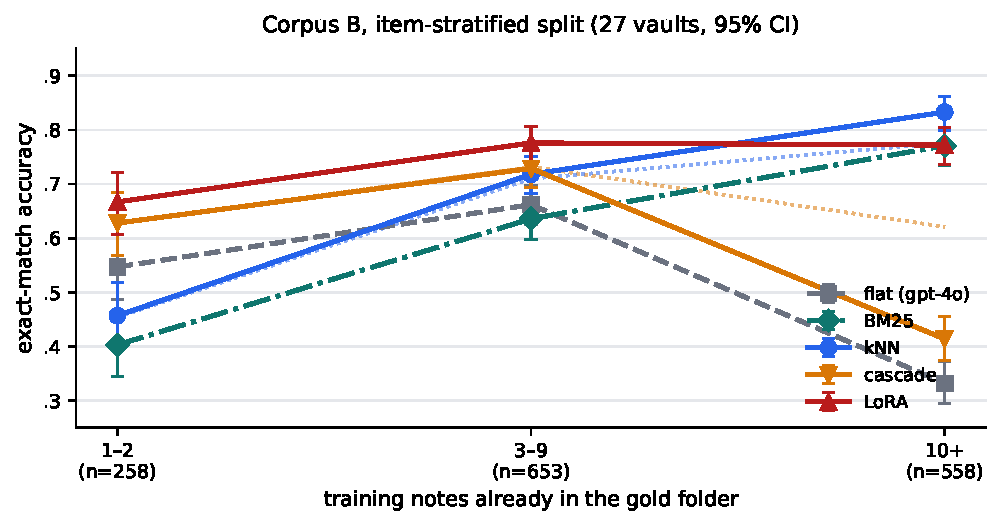
\includegraphics[width=0.86\textwidth]{figures/fig1_coverage_curve.pdf}
  \caption{Exact-match accuracy by occupancy on corpus~\corpB{} (27 public vaults, item-stratified split), with 95\% Wilson intervals. The lines cross. Both retrieval baselines ($k$NN, BM25) rise from the bottom of the sparse bucket to the top of the dense one, while the cascade falls from second place to fourth. LoRA is high and nearly flat. Flat gpt-4o, which sees no training members at all, still moves with the buckets, which is why we treat occupancy as an evaluation axis and not as a cause. Section~\ref{sec:sensitivity} repeats this analysis without three outlier vaults; the crossing survives, the aggregate ranking does not.}
  \label{fig:fig1}
\end{figure}

\begin{table}[t]
  \centering
  \small
  \setlength{\tabcolsep}{5pt}
  \begin{tabular}{@{}lrrrrrrr@{}}
    \toprule
    occ. & $n$ & maj. & flat & BM25 & $k$NN & casc. & LoRA \\
    \midrule
    \multicolumn{8}{l}{\emph{all 27 vaults}}\\
    1--2  & 258 & 0.000 & 0.547 & 0.403 & 0.457 & 0.628 & \textbf{0.667} \\
    3--9  & 653 & 0.064 & 0.662 & 0.636 & 0.718 & 0.729 & \textbf{0.776} \\
    10+   & 558 & 0.545 & 0.332 & 0.771 & \textbf{0.833} & 0.414 & 0.772 \\
    all   & 1{,}469 & 0.235 & 0.516 & 0.646 & 0.716 & 0.592 & \textbf{0.756} \\
    \midrule
    \multicolumn{8}{l}{\emph{excluding 3 outlier vaults} (\S\ref{sec:sensitivity})}\\
    1--2  & 240 & 0.000 & 0.542 & 0.408 & 0.454 & 0.629 & \textbf{0.671} \\
    3--9  & 604 & 0.070 & 0.662 & 0.627 & 0.710 & 0.732 & \textbf{0.781} \\
    10+   & 335 & 0.510 & 0.445 & 0.708 & 0.776 & 0.621 & \textbf{0.806} \\
    all   & 1{,}179 & 0.181 & 0.576 & 0.606 & 0.677 & 0.679 & \textbf{0.766} \\
    \bottomrule
  \end{tabular}
  \caption{Corpus~\corpB{}, item-stratified split. Cascade is gpt-4o over a note-embedding top-20. $k$NN and BM25 use $k{=}5$. ``maj.'' is the majority-class floor. Bold marks the row maximum. The \emph{all} row is the number a conventional paper would report; the rows above it are what that number averages over. The lower block repeats the analysis with the three vaults of \S\ref{sec:sensitivity} removed.}
  \label{tab:corpusb}
\end{table}

Figure~\ref{fig:fig1} and Table~\ref{tab:corpusb} are the main result, and three things are worth separating.

\paragraph{The ranking is not constant.}
In the sparse bucket the order is LoRA $0.667$, cascade $0.628$, flat $0.547$, $k$NN $0.457$, BM25 $0.403$.
In the dense bucket it is $k$NN $0.833$, LoRA $0.772$, BM25 $0.771$, cascade $0.414$, flat $0.332$.
Both retrieval baselines climb from the bottom of the table to the top, and the cascade falls from second to fourth while losing $21$ points in absolute terms.
LoRA is high and nearly flat throughout, which is its own kind of finding.
A reader given only the pooled row would conclude that LoRA is the method and $k$NN is a respectable second; the stratified rows say the two are separated almost entirely by what happens in folders that are nearly empty.

\paragraph{Retrieval alone beats the cascade, but only on this corpus composition.}
Embedding $k$NN at $0.716$ and BM25 at $0.646$ both exceed the gpt-4o cascade at $0.592$ in aggregate, and swapping the picker for Llama-3.3-70B on an identical recipe gives $0.523$, so the aggregate loss is not specific to one API.
That comparison, however, does not survive the sensitivity analysis in \S\ref{sec:sensitivity}: with three vaults removed the same aggregate becomes a tie ($k$NN $0.677$ vs.\ cascade $0.679$), and BM25 falls below the cascade.
We therefore state the aggregate claim narrowly.
A retrieval-only baseline is competitive enough that omitting it can invert a paper's conclusion, which is the reason to require it; whether it \emph{wins} depends on how many dense, label-skewed vaults the corpus happens to contain.

\paragraph{Dense buckets are partly label skew.}
The majority-class column is not a flat floor.
Always predicting the single most frequent training path scores $0.545$ in the $10{+}$ bucket, above flat gpt-4o's $0.332$ there.
Some of what looks like strong dense-bucket performance is a concentrated label distribution rather than filing skill, and any method that can exploit frequency will benefit.
This is a further reason to read the strata as regimes rather than as difficulty levels.

\paragraph{Occupancy is confounded, and we say so.}
Flat gpt-4o cannot see training members at all, yet it still swings $0.547 \rightarrow 0.662 \rightarrow 0.332$ across the same three buckets.
Whatever the buckets are capturing, part of it is folder and vault difficulty, not evidence available to the model.
We therefore report occupancy as an axis along which rankings change, and explicitly do not claim that occupancy \emph{causes} the changes.
Flat gpt-4o is the negative control that forces that caution.

\subsection{Does the crossing depend on a few vaults?}
\label{sec:sensitivity}

The cascade's dense-bucket score is not evenly distributed.
Three vaults account for most of it: \texttt{anthonyamar} (cascade $0.000$ vs.\ $k$NN $1.000$ at $10{+}$), \texttt{satan1a/TheRoadOfSO} ($0.023$ vs.\ $0.795$), and \texttt{ManadayM} ($0.280$ vs.\ $1.000$).
In \texttt{TheRoadOfSO} the folder names are opaque hexadecimal strings, and the cascade responds by naming the gold folder's \emph{parent} instead of the folder itself.
A pooled result driven by three vaults with a shared pathology is a weak result, so we recomputed the whole table without them.
The lower block of Table~\ref{tab:corpusb} is that recomputation, and it removes $40\%$ of the dense bucket.

Three things follow.

First, \textbf{the crossing survives}.
The cascade beats $k$NN by $17.5$ points in the sparse bucket ($0.629$ vs.\ $0.454$) and loses to it by $15.5$ points in the dense bucket ($0.621$ vs.\ $0.776$).
The full-corpus swing of $59$ points falls to $33$, but the sign flip, which is the claim, is intact.
Method ranking still depends on occupancy after the outliers are gone.

Second, \textbf{the aggregate retrieval-beats-cascade result does not survive}, as noted above.
It was carried by these three vaults.

Third, \textbf{the parent-naming pathology is confined to them}.
The share of cascade predictions that are a proper prefix of the gold path is $14.3\%$ in the dense bucket across all vaults but only $2.4\%$ once the three are removed, against $6.7\%$ and $2.6\%$ in the sparse and mid buckets.
So this is a data-quality artifact of a few vaults with uninformative folder names, not a general failure mode of retrieve-then-pick, and we do not present it as one.

One ranking flips under the trim and should be read as unstable: at $10{+}$, $k$NN leads on the full corpus ($0.833$ vs.\ LoRA $0.772$), while LoRA leads once the three vaults are removed ($0.806$ vs.\ $0.776$).
Which retrieval-flavoured method is best in dense folders is not settled by this data.
That the cascade is not the best one is.

\subsection{Public vaults, folders never used}

On the folder-disjoint split of the same 27 vaults ($n{=}1{,}879$), the ordering inverts: cascade $0.583$, flat gpt-4o $0.543$, Llama cascade $0.499$, LoRA $0.475$, $k$NN $0$.

This is the regime where the cascade earns its keep.
Retrieval over notes has nothing to vote for, so the shortlist must be built from path strings, and a model that reads twenty candidate paths and reasons about which one fits does better than a fine-tune that has memorised a tree it is no longer being asked about.
The retrieve-then-pick win is real, and it is confined to unseen folders.
It is not a general fact about cascades versus fine-tunes, which is precisely the claim a pooled number would license.

\subsection{The ranking does not travel between corpora}
\label{sec:reversal}

\begin{table}[t]
  \centering
  \small
  \setlength{\tabcolsep}{4pt}
  \begin{tabular}{lccccc}
    \toprule
    corpus & LoRA & casc. & $k$NN & BM25 & wins \\
    \midrule
    \corpA{} (1 tree)     & 0.537 & \textbf{0.643} & 0.524 & 0.442 & --- \\
    \corpB{} (27)  & \textbf{0.756} & 0.592 & 0.716 & 0.646 & 19/6/2 \\
    \corpAp{} (16) & 0.716 & 0.552 & \textbf{0.732} & 0.666 & 13/3/0 \\
    \bottomrule
  \end{tabular}
  \caption{Item-stratified exact match across all three corpora. $k$NN is $k{=}5$ on \corpA{} and \corpB{}, $k{=}12$ on \corpAp{} (each corpus's own peak). Cascade is gpt-4o. The final column counts vaults won by LoRA / cascade / tied, so the reversal can be checked against something other than a pooled mean.}
  \label{tab:crosscorpus}
\end{table}

Table~\ref{tab:crosscorpus} is the uncomfortable result.
The cascade wins on the private tree.
On both public corpora it loses to LoRA and to $k$NN, and the LoRA-over-cascade win is broad at the vault level (19 of 27 vaults, and 13 of 16), so it is not a pooled-average artifact.
Corpus~\corpAp{} is a different genre entirely, software repositories rather than personal vaults, and it reproduces the same aggregate reversal.

\paragraph{The mechanism we tested, and why it failed.}
The natural explanation is tree size.
LoRA sees the whole folder list; the cascade sees twenty candidates.
In a 39-folder vault those are nearly the same list, and in a 365-folder tree they are not, so smaller trees should favour LoRA.
We first tested this by pooling all 1{,}469 items into three terciles by folder count and running a paired test in each.
The result was a clean monotone dose-response, replicated across both public corpora, with $p$-values down to $10^{-25}$.

It was wrong.
Items within a vault are not independent draws, so pooling them and testing per bin is pseudo-replication: the real number of independent units is 27 vaults, not 1{,}469 items.
Redone at the correct unit, as a permutation test on the Spearman correlation between $\log$ folder count and each vault's own (LoRA $-$ cascade) margin, the effect vanishes:
\corpB{} $\rho{=}{+}0.029$, $p{=}0.887$ ($n{=}27$);
\corpAp{} $\rho{=}{-}0.115$, $p{=}0.669$ ($n{=}16$);
pooled $\rho{=}{+}0.034$, $p{=}0.826$ ($n{=}43$).
Null in both corpora, opposite-signed between them.
We retract the tree-size mechanism.

We report the retraction rather than quietly dropping it because the failure mode is generic to this literature: any corpus built as a set of per-user trees invites item-pooled tests, and item-pooled tests on clustered data will manufacture significance from vault identity.
The same caution applies to the item-level $p$-values elsewhere in this paper; the vault-level win counts in Table~\ref{tab:crosscorpus} are the trustworthy summary.

The reversal itself survives.
Its cause is open.
Two confounds we have not separated are pooled cross-vault LoRA training (one adapter per corpus, not one per tree) and candidate-set size, which is entangled with tree size by construction.

\subsection{Case study: one private tree}
\label{sec:corpusa}

\begin{table}[t]
  \centering
  \small
  \begin{tabular}{lrrrr}
    \toprule
    occupancy & $n$ & flat & $k$NN & LoRA \\
    \midrule
    0     & 353 & 0.354 & 0.000 & 0.363 \\
    1--2  & 18  & 0.278 & 0.444 & 0.222 \\
    3--9  & 105 & 0.200 & 0.381 & 0.371 \\
    10+   & 171 & 0.339 & 0.620 & 0.673 \\
    \bottomrule
  \end{tabular}
  \caption{Corpus~\corpA{}. The occupancy-$0$ row is a \emph{separate} folder-disjoint experiment with its own cascade configuration and its own LoRA checkpoint; $k$NN is zero there by construction. The $1$--$2$ row is $n{=}18$ and its ordering should be read as noise.}
  \label{tab:coverage}
\end{table}

Corpus~\corpA{} is one person's directory and generalises to nothing, but it is where this project started and it is the only corpus with a gold-label check, so we report it in full.

Within the item-stratified split the cascade wins the pool at $0.643$, against LoRA $0.537$, $k$NN $0.524$, BM25 $0.442$, flat gpt-4o $0.286$, and a majority-class floor of $0.061$.
An untrained 8B base model scores $0.051$, and most of the LoRA's gain over that base is schema compliance rather than filing skill: invalid paths fall from $24.8\%$ to $0.7\%$.
Constrained decoding without training did not substitute for the fine-tune.
On the folder-disjoint split, a cascade with a path@50 shortlist scores $0.419$ against LoRA $0.363$ and flat $0.354$.

Table~\ref{tab:coverage} shows the same non-monotone shape as corpus~\corpB{}: flat gpt-4o's best bucket is $10{+}$ and its worst is $3$--$9$, and $k$NN climbs steadily while flat does not.
Item-level paired tests on this corpus describe one tree, and we do not treat them as a population result.
Section~\ref{sec:reversal} is the test at the population unit, and the ranking here does not survive it.

\subsection{What the cascade's gain actually comes from}
\label{sec:grounding-pointer}

A $2\times2$ on corpus~\corpA{} separates the cascade's two differences from flat prompting --- a
shorter candidate list, and selection of which candidates survive. Shortlisting carries the whole
measurable gain ($+35$ points, $p{<}10^{-22}$); attaching a one-line description to each folder is
within noise ($p{\approx}0.49$). The candidate-set factor is bundled, so this is not a clean
mechanism claim; Appendix~\ref{app:grounding} gives the full result and its caveats.

\subsection{Are the gold labels any good?}
\label{sec:annotation}

Exact match against the folder of record only means something if the folder of record is a sensible destination.
Two annotators independently judged 100 notes sampled from corpus~\corpA{}, stratified to match the occupancy buckets, shown only the note text and the recorded folder and never model output.
Cohen's $\kappa$ is $0.901$ on the 98 shared items, with 95 of 98 exact-verdict agreements, and no item was called correct by one annotator and wrong by the other.
Counting ambiguous as a confirmed label, $82$--$94\%$ of sampled gold paths are sensible; Appendix~\ref{app:annotation} gives the per-verdict counts.

Disagreement concentrates in the sparse bucket: $56\%$ clean agreement there against $91\%$, $76\%$, and $91\%$ elsewhere.
Sparse folders are genuinely harder to adjudicate, which means part of the sparse-bucket accuracy drop on corpus~\corpA{} may be label ambiguity rather than method failure.
This study covers corpus~\corpA{} only; \corpB{} and \corpAp{} were not annotated.

% ============================================================================
\section{Discussion and Limitations}
\label{sec:discussion}

Reporting by occupancy changes what the results say.
On public vaults with folders already in use, a retrieval index is a strong method and putting an LLM picker on top of it is not reliably better; on the full corpus it is visibly worse, and after trimming three outlier vaults it is a tie.
That the comparison moves this much under a three-vault trim is itself the argument for reporting strata and sensitivity together rather than a single pooled score.
Fine-tuning wins those vaults in aggregate and still loses to the cascade the moment the folder has never been used.
A private tree produced the opposite headline from both.
Any single accuracy for this task is a mixture over those regimes, weighted by a corpus composition nobody reports.

\paragraph{Limitations.}
Occupancy is confounded with folder, vault, and corpus identity; flat gpt-4o is the negative control that makes this visible, and we do not claim causation.
Corpus~\corpA{} is 78\% one project.
Nine of 25 \corpAp{} clones timed out, and nine of 27 \corpB{} vaults were capped at 250 notes in filesystem order.
Depth caps are not matched across corpora.
LoRA training on \corpB{} and \corpAp{} pools rows across trees rather than fitting one adapter per tree.
Both $k$ and shortlist size were chosen on the validation sets we report.
Item-pooled significance tests in this paper are pseudo-replicated and vault-level counts should be preferred.
A cross-vault leakage check found a near-duplicate training note for 7 of 2{,}266 validation items ($0.31\%$), all traced to one plugin's auto-generated placeholder file.
We score the folder of record, not downstream QA \citep{filesystem-memory}, and not unique correctness (\S\ref{sec:annotation}).

\paragraph{What would settle the open question.}
Two experiments would separate the confounds behind the reversal: per-vault LoRA adapters, to separate training volume from tree structure, and a lexical baseline placed inside the cascade shortlist, to separate retrieval from picking more cleanly than the corpus-\corpA{} $2\times2$ manages.
Neither is required for the recommendation below, which is why we make the recommendation and leave the mechanism open.

% ============================================================================
\section{Conclusion}

Note-placement papers should stop leading with one accuracy.
Report accuracy by occupancy, include a retrieval-only baseline, and include an evaluation on folders that have never been used.
Under that protocol, a retrieve-then-pick cascade is not a general winner, a small fine-tune is not a general winner, retrieval baselines that cost nothing per note are competitive wherever folders are full, and the ranking measured on one private tree does not predict the ranking on public vaults.
We leave the cause of that reversal open rather than attach an explanation the data do not support.

% Acknowledgments omitted: double-blind submission.

\section*{Reproducibility}

Code, corpus manifests with pinned commit SHAs, and the complete run record, including the
corrections and negative results along the way, will be released publicly on acceptance, and are
available to reviewers on request through the programme chairs.
Third-party note text is not redistributed; the manifests rebuild corpora~\corpB{} and \corpAp{}
from their pinned commits, and every table rebuilds from stored per-item artifacts with no API calls.

\bibliographystyle{plainnat}
\bibliography{main}

\appendix
\section{Gold-label annotation counts}
\label{app:annotation}

The annotators were asked one question: is this a sensible home for this note?
Table~\ref{tab:annotation} gives their verdict counts.

\begin{table}[h]
  \centering
  \small
  \begin{tabular}{lcccc}
    \toprule
    & correct & ambig. & unclear & wrong \\
    \midrule
    annotator 1 & 80/98  & 12/98 & 6/98 & 0/98 \\
    annotator 2 & 82/100 & 10/100 & 8/100 & 0/100 \\
    \bottomrule
  \end{tabular}
  \caption{Corpus~\corpA{} gold-label study. Annotator 1 judged 98 unique notes after two duplicated sample rows collapsed.}
  \label{tab:annotation}
\end{table}

\section{What the cascade's gain actually comes from}
\label{app:grounding}

The cascade differs from flat prompting in two ways at once: it shortens the candidate list, and it selects which candidates survive.
A $2\times2$ on corpus~\corpA{}'s item split ($n{=}294$) crosses candidate-set size (all 365 folders vs.\ a retrieved top-20) with a one-line description attached to each folder.

Shortlisting is worth $+35$ points in both description conditions ($p{<}10^{-22}$).
Adding descriptions is within noise in both rows ($p{\approx}0.49$).
So the measurable gain is carried by the candidate set, not by describing what each folder contains.

Two caveats keep this from being a clean mechanism claim.
The candidate-set factor is itself bundled: changing it changes what was retrieved, how many options remain, and how long the prompt is, all together.
And our descriptions are gpt-4o-mini one-liners built from at most four truncated training notes, which is not the same thing as PaperRouter-Agent's inspector reading actual member documents at inference time.
This result is consistent with retrieval carrying the gain we can measure; it does not identify which stage of their pipeline produces their $+22$ points.

\section{Separating personal vaults from software repositories}
\label{app:classifier}

Corpus~\corpB{} starts from GitHub repositories that pass structural note-vault heuristics: note count, directory count, depth, and folder-size spread.
Of the 132 repositories that passed, 95 turned out to be software projects that ship markdown documentation.

The obvious discriminator does not work.
Markdown-to-total-file ratio is $0.41$ on a real vault in our sample and $0.51$ on a real software repository, because vaults carry image and PDF attachments that dilute their markdown share.
What does separate them is the presence of a package manifest (\texttt{package.json}, \texttt{pyproject.toml}, \texttt{Cargo.toml}, and similar) or more than 30 source files.
The filter was checked by hand against known cases during construction; it was not evaluated against a held-out labelled set, so its error rate is unmeasured.
The 95 rejected software repositories became the pool from which corpus~\corpAp{} was later drawn.

\end{document}
